\documentclass{article}
\usepackage{amsmath}
\usepackage{tikz}
\usetikzlibrary{decorations.markings}

\begin{document}

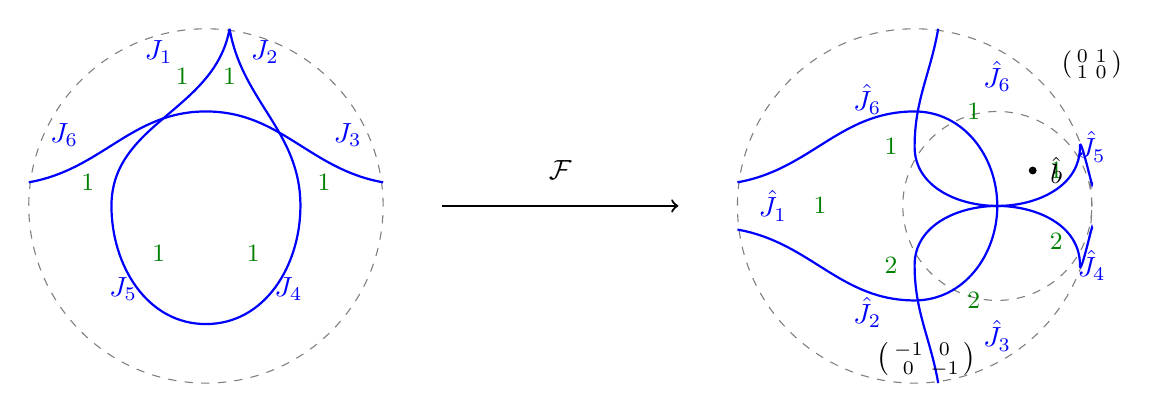
\begin{tikzpicture}[scale=1.5]
    % Define styles
    \tikzset{
        bluecurve/.style={blue, thick},
        greylabel/.style={gray, dashed, thin},
        greennum/.style={green!50!black, font=\small},
    }
    
    % LEFT DIAGRAM (before Fourier transform)
    \begin{scope}[shift={(-3,0)}]
        % Dashed circle
        \draw[greylabel] (0,0) circle (1.5);
        
        % Curves
        \draw[bluecurve] (0.2,1.5) to[out=-100,in=90] (-0.8,0) to[out=-90,in=180] (0,-1) to[out=0,in=-90] (0.8,0) to[out=90,in=-80] (0.2,1.5);
        \draw[bluecurve] (-1.5,0.2) to[out=10,in=180] (0,0.8) to[out=0,in=170] (1.5,0.2);
        
        % Labels for curves
        \node[blue] at (-0.4,1.3) {$J_1$};
        \node[blue] at (-1.2,0.6) {$J_6$};
        \node[blue] at (-0.7,-0.7) {$J_5$};
        \node[blue] at (0.7,-0.7) {$J_4$};
        \node[blue] at (1.2,0.6) {$J_3$};
        \node[blue] at (0.5,1.3) {$J_2$};
        
        % Green numbers (strand numbering)
        \node[greennum] at (-0.2,1.1) {1};
        \node[greennum] at (-1.0,0.2) {1};
        \node[greennum] at (-0.4,-0.4) {1};
        \node[greennum] at (0.4,-0.4) {1};
        \node[greennum] at (1.0,0.2) {1};
        \node[greennum] at (0.2,1.1) {1};
    \end{scope}
    
    % RIGHT DIAGRAM (after Fourier transform)
    \begin{scope}[shift={(3,0)}]
        % Dashed circles
        \draw[greylabel] (0,0) circle (1.5);
        \draw[greylabel] (0.7,0) circle (0.8);
        
        % Curves
        \draw[bluecurve] (-1.5,0.2) to[out=10,in=180] (0,0.8) to[out=0,in=90] (0.7,0) to[out=-90,in=0] (0,-0.8) to[out=180,in=-10] (-1.5,-0.2);
        \draw[bluecurve] (0.2,1.5) to[out=-100,in=90] (0,0.5) to[out=-90,in=180] (0.7,0) to[out=0,in=-90] (1.4,0.5) to[out=90,in=-80] (1.5,0.2);
        \draw[bluecurve] (0.2,-1.5) to[out=100,in=-90] (0,-0.5) to[out=90,in=180] (0.7,0) to[out=0,in=90] (1.4,-0.5) to[out=-90,in=80] (1.5,-0.2);
        
        % Labels for curves
        \node[blue] at (-0.4,0.9) {$\hat{J}_6$};
        \node[blue] at (-1.2,0) {$\hat{J}_1$};
        \node[blue] at (-0.4,-0.9) {$\hat{J}_2$};
        \node[blue] at (0.7,-1.1) {$\hat{J}_3$};
        \node[blue] at (1.5,-0.5) {$\hat{J}_4$};
        \node[blue] at (1.5,0.5) {$\hat{J}_5$};
        \node[blue] at (0.7,1.1) {$\hat{J}_6$};
        
        % Green numbers (strand numbering)
        \node[greennum] at (-0.2,0.5) {1};
        \node[greennum] at (-0.8,0) {1};
        \node[greennum] at (-0.2,-0.5) {2};
        \node[greennum] at (0.5,-0.8) {2};
        \node[greennum] at (1.2,-0.3) {2};
        \node[greennum] at (1.2,0.3) {1};
        \node[greennum] at (0.5,0.8) {1};
        
        % Matrices
        \node at (1.5,1.2) {$\left(\begin{smallmatrix} 0 & 1 \\ 1 & 0 \end{smallmatrix}\right)$};
        \node at (0.1,-1.3) {$\left(\begin{smallmatrix} -1 & 0 \\ 0 & -1 \end{smallmatrix}\right)$};
        
        % Base point
        \node[fill=black, circle, inner sep=1pt] at (1,0.3) {};
        \node at (1.2,0.3) {$\hat{b}$};
    \end{scope}
    
    % Arrow between diagrams
    \draw[->, thick] (-1,0) -- (1,0);
    \node at (0,0.3) {$\mathcal{F}$};
    
\end{tikzpicture}

\end{document}